\documentclass{article}
\usepackage{listings}
\usepackage{graphicx}
\usepackage{float}
\usepackage{fontspec}
\setsansfont{Ubuntu}% Ubuntu as sans - use \sffamily or \textsf{} as normal
\setmonofont{JetBrainsMono Nerd Font Mono}% Ubuntu Mono as 'typewriter' - use \ttfamily or \texttt{}
\usepackage[a4paper,
            bindingoffset=0.2in,
            left=1cm,
            right=1cm,
            top=1in,
            bottom=1in,
            footskip=.25in]{geometry}
\usepackage{hyperref}
\hypersetup{
    colorlinks, citecolor=black, filecolor=black,
    linkcolor=black, urlcolor=black
}
\usepackage{xcolor}
\definecolor{mygreen}{rgb}{0.05,0.15,0.11}
\definecolor{mygray}{rgb}{0.9,0.9,0.9}
\definecolor{mymauve}{rgb}{0.58,0,0.82}
\lstset{
  % backgroundcolor=\color{mygray}, 
  basicstyle=\ttfamily,
  breakatwhitespace=false,
  breaklines=true,
  % commentstyle=\color{darkgray},
  keepspaces=true,
  keywordstyle=\bfseries,
  morekeywords={*,...},
  showspaces=false,
  showstringspaces=false,
  showtabs=false,
  % stringstyle=\color{blue},
  tabsize=4,
  % numbers=left,
  rulecolor=\color{black},
  postbreak=\mbox{\textcolor{red}{$\hookrightarrow$}\space}
}

\begin{document}

\pagenumbering{gobble}
\centerline{\bfseries \Huge Assignment 2}

\section*{Question 1}

WAP in HTML to implement a frame

\begin{figure}[H]
  \caption{Frames}
  \centering
  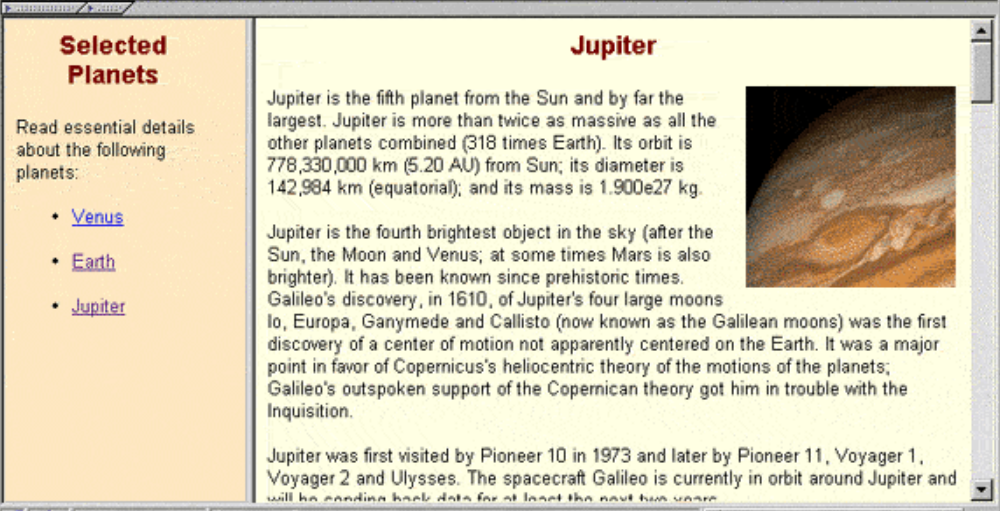
\includegraphics[width=14cm]{./img/1.png}
\end{figure}

\newpage
\subsection*{Code}
\lstinputlisting[language=html]{1/1.html}
\lstinputlisting[language=html]{1/11.html}
\newpage
\subsection*{Output}
\begin{figure}[H]
  \centering
  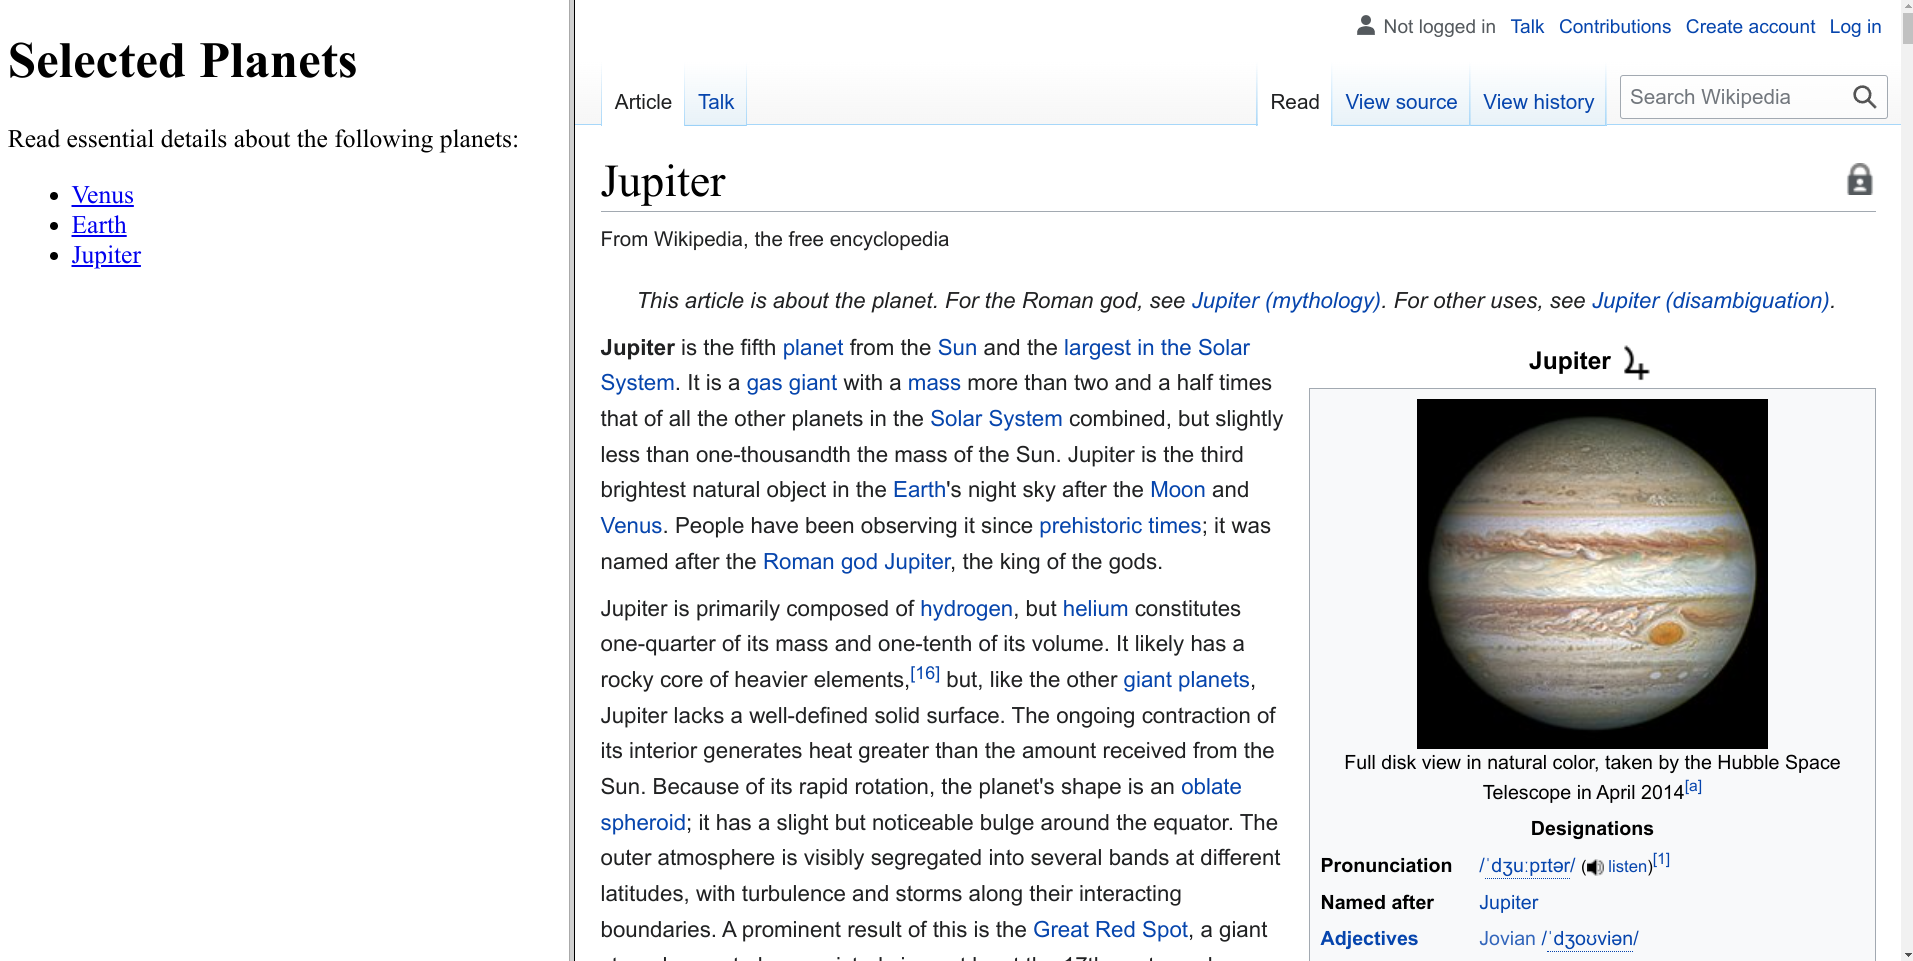
\includegraphics[width=16cm]{1/out.png}
\end{figure}

\newpage
\section*{Question 2}

WAP in HTML to implement a table.

\begin{figure}[H]
  \caption{Table}
  \centering
  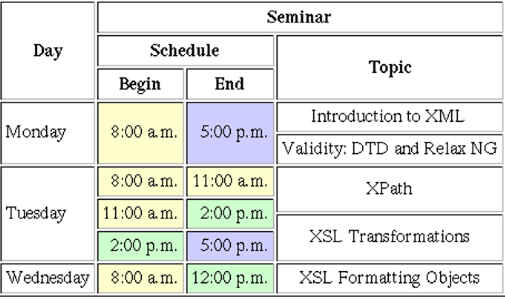
\includegraphics[width=10cm]{./img/2.png}
\end{figure}

\newpage
\subsection*{Code}
\lstinputlisting[language=html]{2/2.html}
\newpage
\subsection*{Output}
\begin{figure}[H]
  \centering
  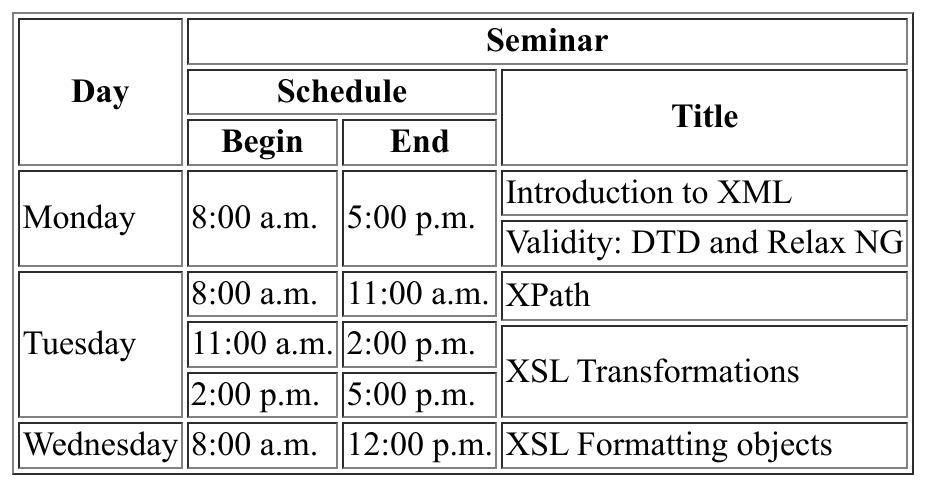
\includegraphics[width=13cm]{2/out.png}
\end{figure}
\end{document}